% Enter the report details below.
\newcommand{\praktikum}{P4} % Lab course P3/P4:
\newcommand{\gruppennummer}{} % Group number:
\newcommand{\gruppentag}{} % Group day (Mo1, Mo2, Mi3):
% Select the matching position for your group day.
\newcommand{\gruppentagposition}{} % Monday group 1 (Mo1)
%\newcommand{\gruppentagposition}{11.7cm,22.8cm} % Monday group 2 (Mo2)
%\newcommand{\gruppentagposition}{13.3cm,22.8cm} % Wednesday group 3 (Mi3)
\newcommand{\semester}{} % Term:
\newcommand{\versuch}{} % Experiment:
\newcommand{\nameeins}{} % Student 1:
\newcommand{\emaileins}{} % Student 1 email:
\newcommand{\namezwei}{} % Student 2:
\newcommand{\emailzwei}{} % Student 2 email:
\newcommand{\assistent}{} % Supervisor:
\newcommand{\durchfuehrungsdatum}{} % Experiment date:
\newcommand{\abgabedatum}{} % Submission date:
%%%%%%%%%%%%%%%%%%%%%%%%%%%%%%%%%%%%%%%%%%%%%%%%%%%%%%%%%%%%%%%%%%%%%%%%%%%%%%%%%%%%%%%%%
% No further editing is required below this line.
\begin{tikzpicture}[remember picture,overlay]
    \node at (current page.center) {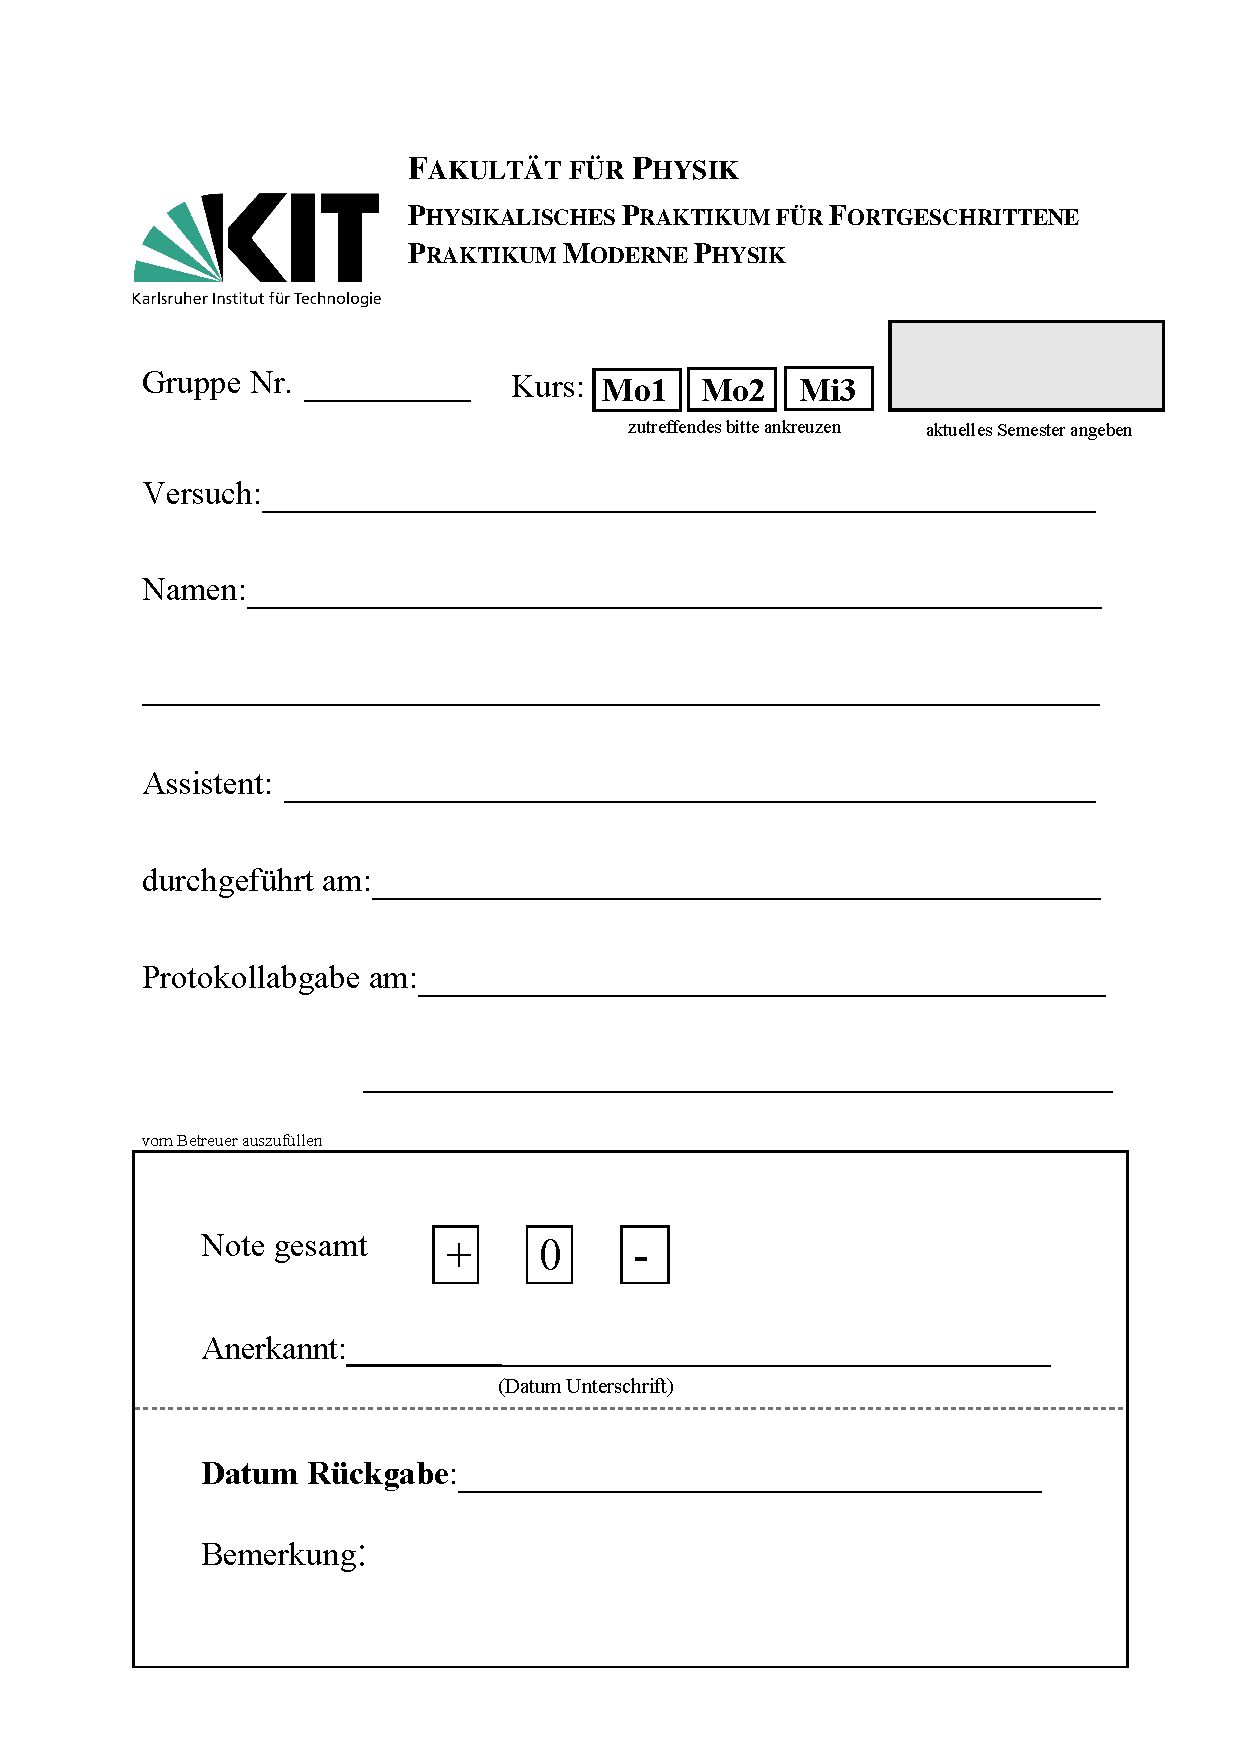
\includegraphics[page=1]{include/Deckblatt.pdf}};
    \begin{scope}[shift={(current page.south west)},every node/.style={anchor=base west}]
        \node at (5.8cm,23.1cm){\Large{\gruppennummer}}; % Group number
        \node at (\gruppentagposition) {\scalebox{4}{{$\mathbf{\times}$}}}; % Group day
        \node at (16cm,23.1cm) {\Large{\semester}}; % Term
        \node at (4.8cm,21.2cm){\Large{\versuch}}; % Experiment
        \node at (4.8cm,19.6cm){\Large{\nameeins\hspace{0.2222em}(\emaileins)}}; % Student 1
        \node at (4.8cm,18.0cm){\Large{\namezwei\hspace{0.2222em}(\emailzwei)}}; % Student 2
        \node at (4.8cm,16.3cm){\Large{\assistent}}; % Supervisor
        \node at (7.2cm,14.6cm){\Large{\durchfuehrungsdatum}}; % Experiment date
        \node at (7.2cm,13.0cm){\Large{\abgabedatum}}; % Submission date
    \end{scope}
\end{tikzpicture}
% Embed report details as PDF metadata.
\hypersetup{
  pdftitle    = {\praktikum\hspace{0.2222em}Lab Report - \versuch},
  pdfsubject  = {Report for experiment \versuch\hspace{0.2222em}on \durchfuehrungsdatum},
  pdfauthor   = {\nameeins\hspace{0.2222em}and\hspace{0.2222em}\namezwei\hspace{0.2222em}(Group \gruppentag-\gruppennummer)},
  pdfkeywords = {KIT, Physics, Laboratory, Lab Report, \praktikum, \versuch, \semester, \nameeins, \namezwei},
  pdfcreator  = {pdflatex},
  pdfproducer = {LaTeX with hyperref}
}